\documentclass{article}
\usepackage{hyperref}
\usepackage{multirow}
\usepackage{array}
\usepackage{xeCJK}
\usepackage{listings}
\lstset{
	basicstyle = \small\ttfamily,
	breaklines = true,
	frame = single,
	language = python,
	tabsize = 2,
	showspaces = false,
	showstringspaces = false,
	breakindent =1.1em,
}
\setCJKmainfont{SimSun}

\title{Y86流水线模拟器的实现\\计算机原理项目报告}
\author{游沛杰 13307130325}
\begin{document}
\maketitle
\tableofcontents
\newpage

\section{背景介绍}
\indent\indent
在本次项目实验中,我们需要实现一个Y86模拟器,能够正确的流水线化模拟执行课本(CS:APP\cite{1})第4章介绍的Y86指令,并将执行过程和程序运行结果通过图形界面的方式可视化。

\section{工作原理}
这里分指令集,流水线阶段,流水线异常处理等部分来介绍
\subsection{指令集}
实现了书本上介绍的全部Y86指令,如下

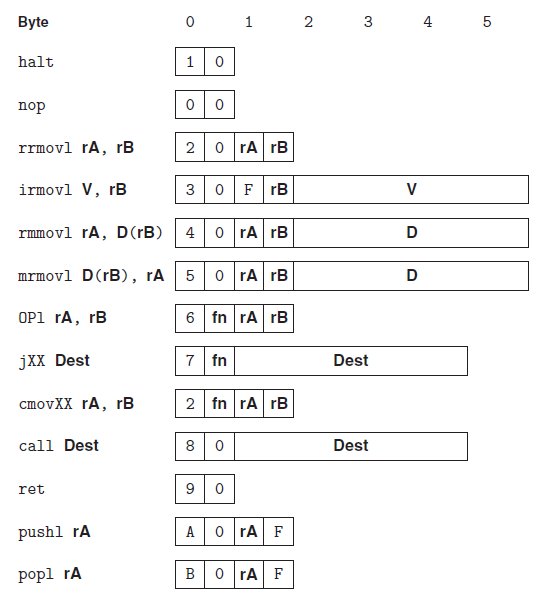
\includegraphics[width = 10cm]{1.png}

其中,地址的形式为D(rB),而指令跳转使用绝对地址的方式(比如jmp 0x123,那么下一条要执行的指令就是0x123开始的指令,而不是pc+0x123或者pc+0x123+0x2)。

另外需要说明的是,书本上的halt和nop对应的机器码不明确(见第二版英文书P338和P384,前后矛盾)。所以在这里,我把10看成是halt指令对应机器码,00看成是nop指令。
\subsection{PIPELINE}
我实现的流水线分成五个阶段(Fetch, Decode, Execute, Memory, Write back)
\begin{enumerate}
\item Fetch      从指令内存中取出指令以及相关信息(rA、rB编号, valC)
\item Decode     读取相关的寄存器的值(rA, rB, RESP的值)
\item Execute    进行算术/逻辑运算
\item Memory     读写内存
\item Write back 将需要更新的寄存器值放回register file中
\end{enumerate}

使用forward+stall/bubble来处理异常情况。
\begin{itemize}
\item forward 将前面阶段中已经计算好的值直接传输到decode阶段
\item stall 不执行更新,但是保留原来流水线寄存器中的值(延迟到以后再更新)
\item bubble 把pipeline register中保存的值重置置为默认值(舍弃当前已在进行的指令操作)
\end{itemize}
\section{我的项目概况}
\begin{center}
\begin{table}[!ht]     % 强制在原位显示表格
\centering
\caption{开发环境}
\begin{tabular}{|l|c|c|c|}
\hline
\multirow{2}{*}{主要使用语言} & 内核 & Python 2.7.9\\
\cline{2-3}
 & GUI & PyQt 4.11.3\\
\hline
\multirow{2}{*}{开发平台} & IDE & PyCharm\\
\cline{2-3}
& 操作系统 & Windows 8.1\\
\hline
辅助工具 & GUI界面绘制 & Qt Creator\\
\hline
\end{tabular}
\end{table}
\end{center}

全部代码均作者本人\underline{独立完成},并没有抄袭和复制粘贴的成分。

项目的设计和准备阶段从5月16日开始,经历两个星期(其中有另外2个项目需要完成)。从6月1日左右开始投入实际开发。其中核心部分历时4天编写并完成调试,UI部分做了4-5天。

在这个项目之前我们还完成了数据库的课程项目(HTML+PHP实现),所以作者这次决定不再写web的UI,试图使用不会的Qt来实现一个桌面端应用程序。虽然界面不一定有HTML+CSS+JavaScript实现的好看,但是也是一种挑战。

%目录介绍here

\section{内核具体实现}
\subsection{中间变量的实现}
这里的中间变量指的的stage output,通常以小写字母fdemw开头(比如e\_valE)。

对于这些结果,在硬件上相当于一个组合电路,那么我们就用一个函数来实现,其中函数的输入就相当于硬件层面上的接线,组合电路就在函数内部实现其功能,比如下面例子:

\begin{lstlisting}[frame=single]
def f_stat(f_icode, imem_error):
    #   DONE
    #   有优先级?
    if imem_error: return SADR
    if not instr_valid(f_icode): return SINS
    if f_icode == IHALT: return SHLT
    return SAOK

\end{lstlisting}

其中部分stage output只用到了一次
%example
,我们在需要的时候再计算这个结果,以保证程序整体运行速度,而对于在不止一个地方用到的值,我们采用中间变量来保存这些值。
%example
\\
\\
\\
\indent 我们可以发现,Python的语法与课本上的HCL有很多相似之处,比如有in的用法,Python的list理解起来也比较简单,如下语句:
\begin{lstlisting}[frame=single]
def d_srcB(D_icode, D_rB):
    #   DONE
    if D_icode in [IOPL, IRMMOVL, IMRMOVL]: return D_rB
    if D_icode in [IPUSHL, IPOPL, ICALL, IRET]: return RESP;
    return RNONE;
\end{lstlisting}

我们发现Python在这里看起来就和真的硬件描述语言一样,同时十分接近自然语言,给人带来愉悦感!这也是类似于C++之类的语言所没有的
%词穷
。

\section{UI介绍}
\section{UI实现}
\section{其他功能}
\section{遇到的问题}
\section{项目总结}
\section{Thank You}
\indent\indent
{\Large{View this project on GitHub\cite{2}}
\\
\\
\indent\Large{Report is written by \LaTeX}}

\begin{thebibliography}{99}
\bibitem{1} \url{http://www.csapp.cs.cmu.edu/}
\bibitem{2} \url{https://github.com/kjkszpj/AE86}
\end{thebibliography}

\end{document}